\problemname{Tournament}

\begin{figure}[h!]
  \centering
  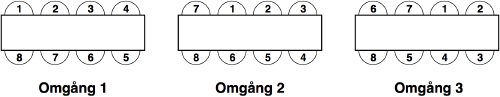
\includegraphics{turnering.png}
\end{figure}

If you want to organize, for example, a table hockey tournament where everyone plays everyone, you can use a practical rotation schedule called round robin.
It works such that in the first round, the players face each other according to the figure above (we assume the number of players $n$ is even).
When the first round is over, all players move one step clockwise, except for the player in the lower-left corner who is skipped (hence the name, you move ``around'' Robin, i.e., the last player).
With this rotation schedule, you are guaranteed that everyone has played everyone exactly once after $n-1$ rounds.

Your task is to write a program that outputs which players face each other in a given round.

\section*{Input}
The input consists of two integers: the number of players in the tournament (an even number $n$ between $2$ and $100$) and the round (between $1$ and $n-1$).

\section*{Output}
The program should output $n/2$ lines describing who plays whom, where each line is in the format \texttt{a-b}.
The order of the matches does not matter.
